Si se quiere desarrollar una aplicación en Android este es una de los puntos más importantes de esta memoria ya que se detallara los puntos más importantes y los problemas que se han tenido al desarrollar la aplicación y problemas que pueden surgir.
Para empezar, lo más importante ¿Por qué programar en Android y no en otro SO?
El motivo por el que Baldugenda está para Android  y no es multiplataforma es que quería centrarme en Android y ver todo el potencial que tiene.
Aparte si hablamos de números podemos ver cómo están actualmente los sistemas operativos en el mercado móvil.

\begin{figure}[H] 
  \begin{center} 
    \scalebox{0.6}{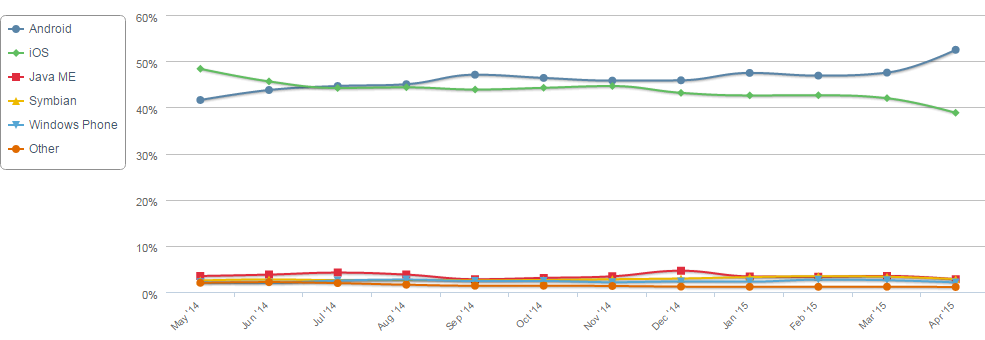
\includegraphics{figs/TendenciasSO.png}} 
    \caption{Tendencias en móviles SO netmarketshare.com} 
    \label{fig:TendenciasSO} 
  \end{center} 
\end{figure}

Se puede ver que a principios de este año Android le ha cogido la delantera a iOS, los dos son líderes en el mercado móvil.
Google ha conseguido resolver la fragmentación de sus versiones de Android y eso le ha dado dolores de cabeza a iOS la cual ha pasado a ocupar el segundo lugar.

\begin{figure}[H] 
  \begin{center} 
    \scalebox{1}{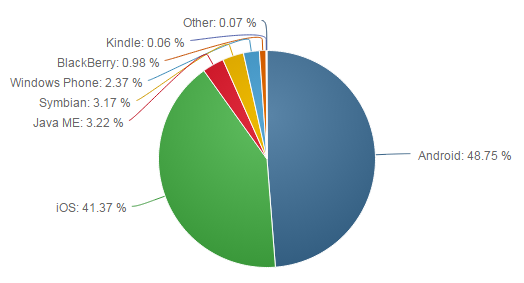
\includegraphics{figs/RankingSO.png}} 
    \caption{Ranking de móviles SO netmarketshare.com} 
    \label{fig:TendenciasSO} 
  \end{center} 
\end{figure}

El motivo anterior sumado al aumento de personas que usan Android en sus dispositivos y siendo yo un usuario de Android en estos momentos me llevo a la decisión de querer sacarle el máximo partido realizando una aplicación nativa en Android.
Antes de comenzar a desarrollar en Android hay ciertos aspectos que hay que saber.
Uno muy importante es que se necesita conocimientos de Java.
Y estar acostumbrado a trabajar con programación orientada a objetos.
Aparte de estos dos anteriores, un IDE que actualmente el que más auge tiene entre los desarrolladores es el Android Studio por su facilidad a la hora de crear un proyecto.
Y muchas ganas de aprender.
Si se tiene todo lo anterior programar en Android no resultara complicado. Al principio parecerá todo un poco lioso pero el periodo de aprendizaje después compensa ya que lo que al principio tardarías en hacerlo 3 horas al cabo de 2 semanas podrás hacerlo en 10 minutos porque ya te sabrás la mayoría de funciones principales en Android.

\subsection{Restricciones de API}
\label{subsecc:Restricciones de API}

Ya he comentado anteriormente que Google ha ganado terreno en el mercado de los móviles por su labor en la desfragmentación de Android, aun con la labor de Google nos seguimos encontrando que si no cogemos las versiones antiguas de Android y solo desarrollamos para las nuevas quitaremos una parte importante de los usuarios.

\begin{figure}[H] 
  \begin{center} 
    \scalebox{1}{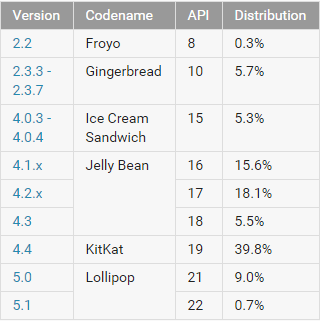
\includegraphics{figs/VersionesAndroid2.png}} 
    \caption{Versiones Android developer.android.com} 
    \label{fig:VersionesAndroid2} 
  \end{center} 
\end{figure}

Estas estadísticas son de mayo de 2015, si se quiere conservar a la mayor cantidad de gente y no limitarse mucho con la aplicación los expertos recomienda empezar a olvidar a la gente que tiene GingerBread para abajo.
En la aplicación de Baldugenda se cogió también a los de API 10 ya que las funciones que se iban a implementar no suponían gran avance tecnológico en cuanto a versión de Android así que se podía usar perfectamente la versión 10 sin verse limitado.
Al coger API más bajas uno se expone a tener que realizar más código especial para esas versiones antiguas e invertir tiempo en retocar cosas para que no se note la diferencia y que el usuario no tenga problemas de interacción.
 
Cada una de las APIs mostradas arriba añade diferentes funciones, la más destacada la se puede ver comparando el API 10 con el API 21, el apartado grafico que usa Android en una u otra varía mucho dependiendo de la versión que se use como mínimo.
Más adelante se explicara la interfaz en Android, pero para ver la diferencia y el coste que aumentaría usar una API de más bajo nivel del necesario, se puede ver en la barra de arriba de los dispositivos móviles. A partir del API 21 Android ha optado por un diseño llamado Material Design, este diseño produce que el usuario vea la aplicación más cercana al trabajar con sombras, distintas profundidades y colores más llamativos.
El problema surge cuando se quiere usar este diseño en APIs más bajas, Google proporciona documentación para realizar el material design sobre versiones anteriores a Lollipop, pero aun y todo con toda esa información la diferencia entre usar un API como la 21 frente a usar un API 10 cambia muchísimo.

\begin{figure}[H] 
  \begin{center} 
    \scalebox{1.2}{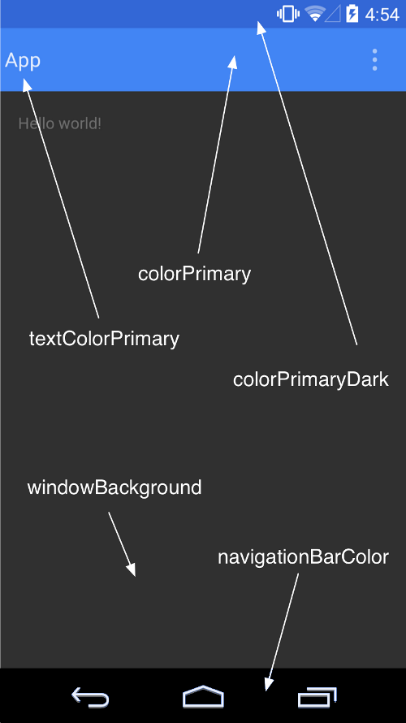
\includegraphics{figs/AndroidToolbar.png}} 
    \caption{Android Toolbar colores android-developers} 
    \label{fig:AndroidToolbar} 
  \end{center} 
\end{figure}

En la imagen mostrada arriba se puede apreciar cómo funcionan los colores en Android desde la versión 21, en cambio si se quiere conseguir algo parecido a eso hay que implementar clases que hagan lo mismo, y no se puede basar solo en las librerías de compatibilidad que ofrece Google.
Un componente que agrego el api 21 fue la toolbar que como se pude ver también permite cambiar el color de la barra donde se encuentra la hora, etc…
En el api 10 el resultado final es muy parecido pero se invierte bastante tiempo, que si el diseño no es primordial, molesta gastarlo agregando colores.

\subsection{Tipo de dispositivos}
\label{subsecc:Tipo de dispositivos}

Android a diferencia de IOS tiene una gama demasiado grande de dispositivos, muchas empresas usan el sistema operativo de Android para sus móviles.
Por este motivo cuando se quiere desarrollar para Android hay que saber muy bien a que dispositivos se quiere dirigir la aplicación.
Los dispositivos Android pasan desde una pantalla de televisión, hasta un pequeño smartwatch.
Hay que saber que dispositivos quitar para llegar a la mayor parte de los usuarios que se quiere que usen la aplicación.
Para resolver la duda Google ofrece periódicamente las estadísticas de los dispositivos usados y sus versiones.
De las versiones ya se ha hablado en un tema anterior, ahora en este apartado se hablara de las densidades y los tipos de pantalla.

\begin{figure}[H] 
  \begin{center} 
    \scalebox{0.7}{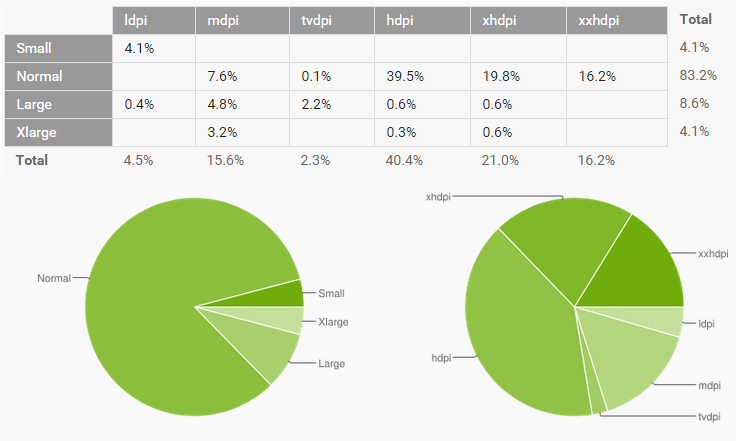
\includegraphics{figs/ComparativaPantallas.png}} 
    \caption{Comparativa tipo de pantallas developer.android.com} 
    \label{fig:ComparativaPantallas} 
  \end{center} 
\end{figure}

Estos datos los proporciona Google, actualizado en mayo de 2015.
Se puede apreciar las distintas gamas que hay de dispositivos. A la hora de crear el proyecto si se usa Android Studio te ayudara un poco con estos temas preguntándote hacia que dispositivo va destinada la aplicación y tendrás que elegir entre móviles o tablets, televisión, aparatos wear de Android, o las Google glass.
Dependiendo de la elección se escoja en ese momento se modificaran automáticamente los ajustes para que esté preparado para el dispositivo seleccionado.
Baldugenda es una aplicación destinada a móviles y tablets ya que su uso está pensado para ser algo habitual y de acceso rápido.
Las aplicaciones que se desarrollan del estilo de Baldugenda suelen ser para móviles también ya que tienen que hacer la función de agenda virtual. Eso no quita para que también haya widgets de esas aplicaciones compatibles con dispositivos como los smartwatch donde se reciben las notificaciones de las aplicaciones de este género.

\subsection{Interfaz}
\label{subsecc:Interfaz}

Uno de los problemas más grandes que se encuentra uno al desarrollar en Android y en cualquier sistema operativo para dispositivos móviles es la limitación de espacio en la pantalla de aparato, también al haber distintos tipos de pantallas hacerlo compatible con todos es una tarea ardua.
Hay muchos aspectos que hacen que los usuarios no borren la aplicación, como puede ser que les parezca entretenida o útil, pero por mucho que una aplicación cumpla todo eso por debajo, a los usuarios se les gana por la vista. Si se quiere mantener la aplicación instalada en los dispositivos de los usuarios tiene que ser agradable para la vista y también cómoda de usar.
De algo que pecamos la mayoría de los informáticos es que el diseño no corre por nuestras venas y por muy divertida que hagamos la parte lógica de la aplicación después el diseño se resiste a salir bien.
Pero aun y todo evitando este tema hay que dedicarle un tiempo después de haber finalizado la parte lógica y antes de publicar la aplicación al apartado de diseño.
Unos colores vivos frente a un fondo blanco marcan la diferencia.
En el caso de Baldugenda durante la primera fase se decidió hacer los casos de uso y que fueran los Baldusers los que dieran propuestas de diseño que les parecen más atractivos.
De esa forma se pasó de un menú principal de 6 botones grises y un fondo blanco a 6 iconos con fondo de colores.
Android proporciona muchos componentes para retocar la interfaz a la hora de desarrollar algunos tan vistosos como un ExpandableList y otros que pasan desapercibidos como puede ser un TextView.
Lo más importante es sacarle provecho a la pequeña pantalla sobre la que se está trabajando y usar dispositivos con pantalla pequeña para realizar las pruebas. Ya que estos casos son los más peligrosos, en el caso de que sobre mucho espacio en un dispositivo de tamaño más grande siempre se podrá meter algo más dependiendo del tamaño pero si tiene la pantalla demasiado pequeña hay que saber comunicar al usuario para que no se pierda en la aplicación.
 
Algo muy vistoso y que no debe faltar en ninguna aplicación son los menús laterales, estos menús no ocupan espacio para el usuario y cuando él quiere los abre y los cierra.
\newpage
\begin{figure}[H] 
  \begin{center} 
    \scalebox{0.7}{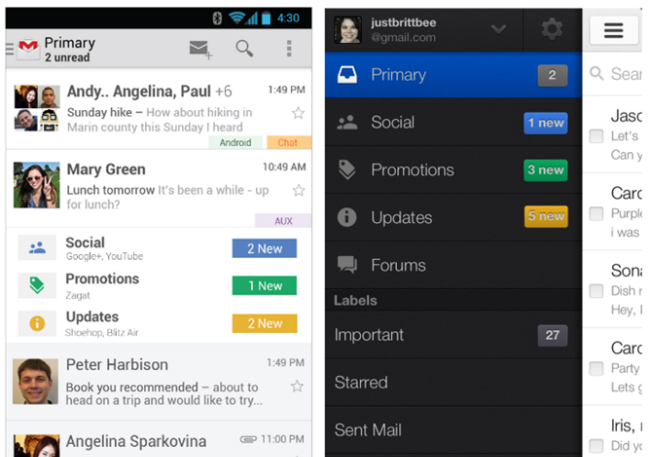
\includegraphics{figs/MenuLateral.png}} 
    \caption{Menu lateral Gmail} 
    \label{fig:MenuLateral} 
  \end{center} 
\end{figure}

En Baldugenda se puso un menú de este tipo en la lista de exámenes y les pareció interesante a los usuarios.
Algo que como desarrolladores hay que aprender es que la aplicación no es para el que la desarrolla que también puede ser pero no principalmente. La aplicación tiene que ir destinada a los usuarios y por este motivo ellos no se van a fijar en la dificultad que tiene sacar la información de la base de datos y mostrarle justo lo que buscan cuando lo buscan.
A ellos lo que les importa principalmente es que sea impactante y divertida a la hora de interactuar con ella.
Si se cambia un botón por algo distinto donde el usuario arrastre o realice otra acción eso le sorprenderá.
El ejemplo que se encontró en Baldugenda es al realizar borrados y modificaciones.
Dependiendo del usuario que la ejecutaba y la edad que tuviera estaban más acostumbrados a las acciones especiales de los botones como mantener pulsado o arrastrar.
Un punto interesante también son los Dialogs, ventanas que se muestran superpuestas a la actividad que se está ejecutando. Gracias a esos dialogs se gana mucho espacio y se consigue que el usuario preste atención a la zona donde se quiere en cada momento.
Volviendo a las pulsaciones largas y juntándolo con el tema de los dialogs en Baldugenda se juntó todo esto y usaron los menús para realizar acciones sobre un objeto en específico.
Los expandable list view es una buena forma de mostrar listas muy largas de lo que se precise agrupándolas por un motivo en concreto.
De esta forma el usuario no tendrá una lista que le ocupa la pantalla, en vez de eso tendrá cajitas que abriendo una tendrá lo que busca de esa categoría.


\begin{figure}[H] 
  \begin{center} 
    \scalebox{0.7}{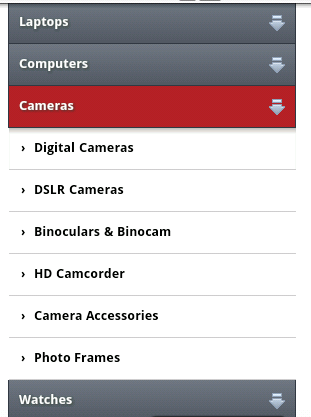
\includegraphics{figs/ExpandableList.png}} 
    \caption{Expandable list view} 
    \label{fig:ExpandableList} 
  \end{center} 
\end{figure}

En este punto también entra el toque artístico de cada persona, cada caja se puede diseñar de la forma que el desarrollador quiera y añadir los colores también.

\subsection{Migración}
\label{subsecc:Migración}

Cuando se decidió implementar en Android se descartó usar aplicaciones para desarrollar multiplataforma. 
Por este motivo hubo que mirar las posibilidades que había y las dificultades que se encontrarían si se tuviera que implementar Baldugenda por ejemplo para IOS o Windows Phone.
Microsoft se ha adelantado a la compañía del Androide y de la manzana y ha optado por ayudar a los desarrolladores a migrar aplicaciones desde IOS y Android a Windows Phone.
Esta medida se debe a las estadísticas que se han podido ver sobre los smartphones y el tipo de sistema operativo que usan. 
Para ello ha ideado una api estilo diccionario para ver las equivalencias entre Android y Windows phone y con eso hacer más fácil a los desarrolladores.
Entre IOS y Android no es tan fácil la cosa. Los dos son empresas muy fuertes en el mercado de los móviles y no darían su brazo a torcer para ayudar a su competidora. 
Pero algo positivo que tiene trabajar con un modelo MVC es que cada apartado está separado.
El modelo se podría trasladar directamente a IOS y la parte de la vista y controlador se podría distribuir entre más personas para desarrollar sobre el ejemplo de Android.
Cuando se habla de migraciones siempre se viene a la cabeza cambio de sistema operativo y cosas así, pero también una migración podría ser el salto de una aplicación móvil a un dispositivo wear de Android o a una pantalla de televisión. Para eso el cambio vendría a ser muy parecido pero pudiendo usar gran parte del código exceptuando cosas como la parte de la vista y la conexión entre la vista y la lógica.
Un punto importante que hay que tener en cuenta a la hora de migrar no es solo instalar la aplicación en un nuevo dispositivo, hay que pensar en los usuarios y permitirles llevarse todo lo realizado hasta el momento en la aplicación anterior a la nueva.
Hay aplicaciones que guardan la información en sus propios servidores y ese paso es transparente para el usuario.
En cambio en el caso de Baldugenda al no usar ningún servidor exceptuando el de Google Calendar para guardar los exámenes, se decidió poder migrar los datos mediante la opción de exportar base de datos y usar la cuenta de Google para pasar de un dispositivo a otro.

\subsection{Notificaciones}
\label{subsecc:Notificaciones}

Las notificaciones en Android es un componente importante dentro de las aplicaciones. Es la forma con la que la aplicación se comunica con el usuario.
Hay distintos tipos de notificaciones:
Están las notificaciones Toast que son mensajes que se escribirán en la pantalla durante un periodo largo o corto según se le indique.
\newpage
\begin{figure}[H] 
  \begin{center} 
    \scalebox{0.7}{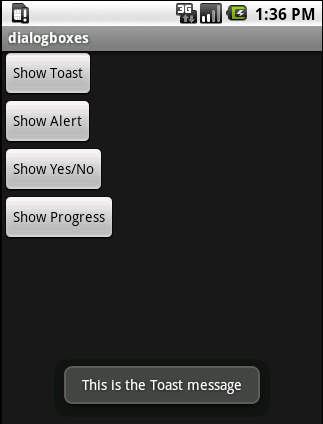
\includegraphics{figs/NotificacionToast.png}} 
    \caption{Notificación Toast} 
    \label{fig:NotificacionToast} 
  \end{center} 
\end{figure}

A la hora de realizar la aplicación si no se encuentra dónde está el fallo, una forma muy útil de usar las notificaciones Toast es sacar por este mensaje los valores que nos interesen para saber si se está trabajando sobre el objeto que se necesita.
Dentro de Baldugenda se ha usado los Toast para comunicar al usuario que se había creado un examen o una asignatura. Hay veces que el teclado tapa estos mensajes así que hay que tener cuidado en qué momento se escriben porque puede que el usuario no lo vea.

Otro tipo de notificaciones son los alertdialog y los timepicker dialog y datepicker dialog.
El alertdialog admite un título, un texto y como máximo 3 botones. Se suele usar para hacer que el usuario confirme una acción, en Baldugenda se ha usado a la hora de borrar la asignatura se le pregunta sí está seguro de borrarla, si pulsa que si la asignatura se borrara en cambio sí cancela no habrá pasado nada.
\newpage
\begin{figure}[H] 
  \begin{center} 
    \scalebox{0.7}{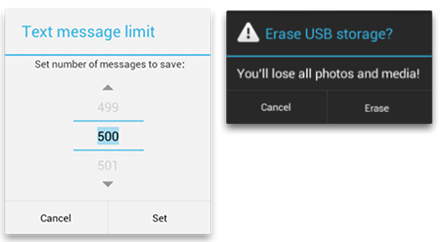
\includegraphics{figs/EjemplosDialog.png}} 
    \caption{Ejemplos de dialog} 
    \label{fig:EjemplosDialog} 
  \end{center} 
\end{figure}

Tanto el timepicker dialog como el datepicker dialog son ventanas modales que actúan sobre la hora y la fecha respectivamente.
Se le da la opción al usuario que escoja el dia mediante el datepicker y mediante el timepicker puede seleccionar la hora.

Dependiendo de la versión del dispositivo estas  ventanas modales serán de una forma u otra.

\begin{figure}[H]
 \centering
  \subfloat[Ejemplo DatePicker en Lollipop]{
   \label{f:Ejemplo DatePicker en Lollipop}
    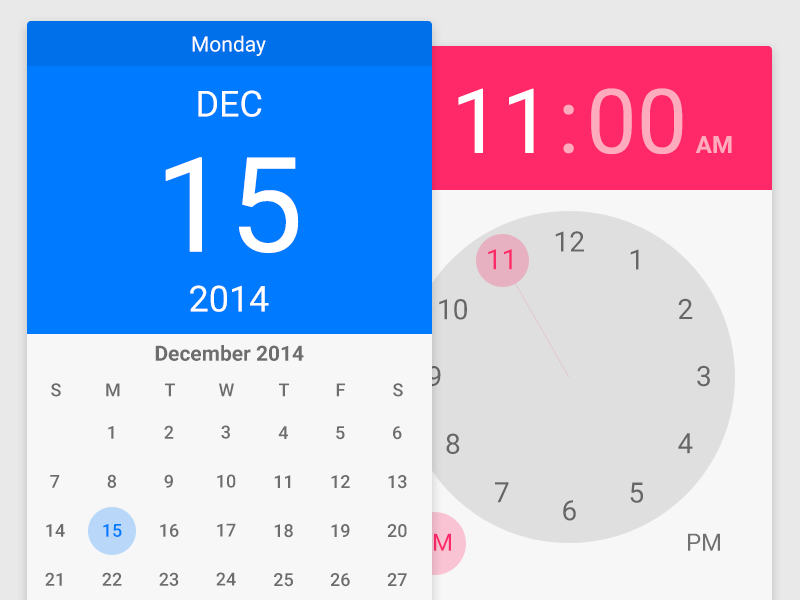
\includegraphics[width=0.4\textwidth]{figs/DatePickerLollipop.png}}
  \subfloat[Ejemplo DatePicker en JellyBean]{
   \label{f:Ejemplo DatePicker en JellyBean}
    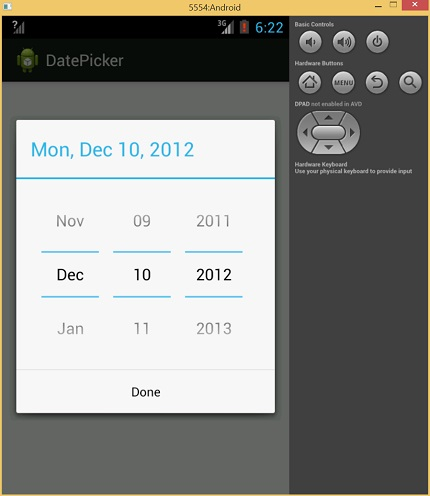
\includegraphics[width=0.4\textwidth]{figs/DatePickerJellyBean.png}}
 \caption{Tipos de DatePicker dependiendo de la version}
 \label{f:Tipos de DatePicker dependiendo de la version}
\end{figure}

A la izquierda podemos ver el datepicker en la versión de lollipop y a la derecha un una versión anterior.
Para el manejo de los días se usa la clase Calendar de java y eso ha venido muy bien ya que Google Calendar sus funciones permiten directamente meter una fecha creada en un objeto Calendar al evento.
De esa forma el trabajo que nos hubiera supuesto tener que sacar la fecha actual calcular cuánto falta hasta la fecha elegida por el usuario y demás, se quita y solo teníamos que sacar la información que seleccionaba el usuario e insertarla en el evento.
Aparte de estas notificaciones tenemos  una muy importante si se va trabajar con servicios de Google que es el progress dialog.
Este tipo de componente es muy útil con estos servicios ya que al usar los servicios de Google hay veces que las conexiones tienen que hacerse en segundo plano y hay que lanzar tareas asíncronas, pero se sigue dependiendo del resultado del servicio para seguir trabajando.
Con este componente se genera una barra de progreso que se ira rellenando según avance la tarea asíncrona o directamente un mensaje que no dejara realizar ninguna otra acción hasta la finalización de la tarea asíncrona.
En Baldugenda se le ha dado uso al realizar la búsqueda de los calendarios y al realizar la creación de exámenes, porque dependiendo de la velocidad que tenga el móvil por internet, puede que el servicio de Google Calendar no vaya lo más rápido que debería y dé error si dejamos que se genere en la ventana secundaria sin avisar al usuario. 

\begin{figure}[H] 
  \begin{center} 
    \scalebox{0.8}{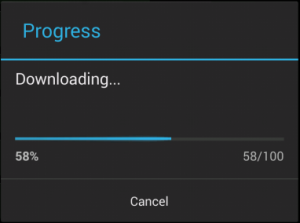
\includegraphics{figs/ProgressDialog.png}} 
    \caption{Ejemplos de ProgressDialog} 
    \label{fig:ProgressDialog} 
  \end{center} 
\end{figure}

Mostrarle al usuario una ventana explicándole lo que está pasando en cada momento hace que no se ponga a pulsar todos los botones pensando que se le ha quedado parada la aplicación.
Se han dado situaciones en el proyecto que por no avisar al usuario que se había generado un examen mediante una ventana de progress dialog, el usuario se pensaba que no estaba generada y la intentaba crear otra vez con el consiguiente error. 
Por eso es una buena opción si se quiere llamar la atención del usuario, si lo comparamos con los toast esta opción es más engorrosa pero el usuario la vera aunque tenga el teclado abierto.

\subsection{Uso de calendarios}
\label{subsecc:Uso de calendarios}

Ya se ha hablado de los timepicker dialog y datepicker dialog en el apartado de las notificaciones de Android.
En este punto se hablara más a fondo del uso que se le suelen dar a los calendarios en las aplicaciones del tipo Baldugenda.
Android tiene un calendario dentro del dispositivo que si no se le asocia ninguna cuenta trabajara con eventos en local. Muchas aplicaciones usan este calendario para generar ahí los eventos, otras simplemente crean su propio calendario dentro de la aplicación.
El problema que se vio al generar el calendario dentro de la aplicación era que el usuario tenía que estar duplicando los eventos si quería tenerlo siempre disponibles.
Una de las mejoras que se tiene pendiente en Baldugenda es la visualización de los eventos en formato mes.

\begin{figure}[H] 
  \begin{center} 
    \scalebox{0.8}{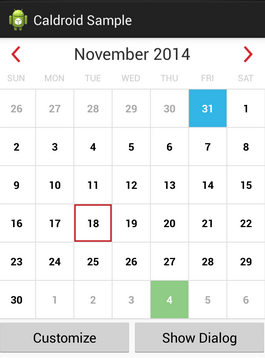
\includegraphics{figs/Caldroid.png}} 
    \caption{Ejemplo de Caldroid Github} 
    \label{fig:Caldroid} 
  \end{center} 
\end{figure}

Como se puede observar en la imagen esa sería un tipo de ventana que se quiere implementar en la aplicación Baldugenda para mostrar por días los exámenes que se tienen apuntados.
Por falta de tiempo no se realizó, aunque si se tenían propuestas librerías para realizar este tipo de vista como puede ser caldroid una librería con copyright disponible en github que ofrece las funciones necesarias y el diseño, para mostrar el calendario de esta forma y poder generar eventos y marcarlos de colores.
Aun y todo se seguiría usando Google Calendar para mantener consistencia a los calendarios del usuario y que tenga acceso siempre a los eventos que se generan dentro del móvil.
Android ofrece su propio componente de vista de calendario, el Calendar view, el problema que se encontró al usarlo es las limitaciones visuales que tiene, se buscaba al usar ese vista mostrar los exámenes que había en el mes, y con Calendar view no se podía agregar eventos a los días del calendario.
Por ese motivo se decidió dejar el tema de la vista del calendario como algo secundario y centrarse en cosas más importantes como el backup
Se ha probado a instalar muchas aplicaciones que tienen la finalidad de guardar asignaturas y exámenes en el móvil junto con sus fechas pero el resultado siempre era el mismo exceptuando alguna que era de pago y que en su versión gratuita no te permitía hacerlo pero en la versión de pago si, las de más aplicaciones funcionaban en local y algunas te daban la posibilidad de exportar los calendarios a la tarjeta sd del móvil por si querías usarlos.
De esta forma se propuso la idea de vincular Google Calendar a la aplicación y darle un toque novedoso.

\subsection{Tareas asíncronas}
\label{subsecc:Tareas asíncronas}

Este punto es muy importante ya que a partir de la versión 4 no se permite realizar peticiones http en el hilo principal de la aplicación, esto tiene sentido ya que significaría ralentizar la aplicación llegando en algunos momentos a bloquearla.
Para esto se crean clases asíncronas que se lanzaran con las llamadas a los servicios que se necesiten.

\begin{figure}[H] 
  \begin{center} 
    \scalebox{0.8}{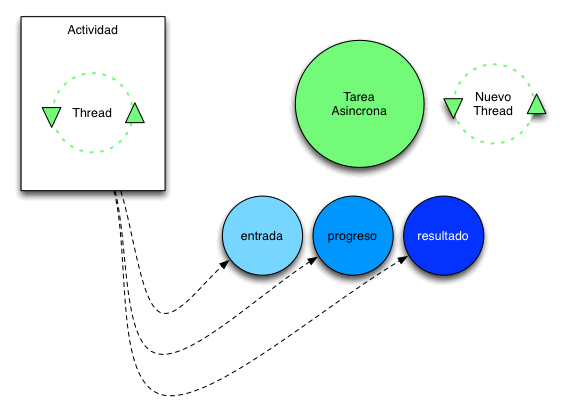
\includegraphics{figs/TareasAsincronas.png}} 
    \caption{Tareas asíncronas android funcionamiento arquitecturajava.com} 
    \label{fig:TareasAsincronas} 
  \end{center} 
\end{figure}

En el apartado de notificaciones se le ha dado importancia a la parte del progres dialog, esto es porque mientras se está ejecutando la tarea asíncrona la actividad sigue funcionando en un thread principal. Por este motivo si se necesita esperar a que la tarea finalice y devuelva el dato a la actividad habría que usar ese progres dialog para que no se permita modificar nada hasta que acabe.
Al extender de la clase AsynTask de Android, obligara a que se tenga que implementar la función de doInbackground, esta función es la que realizara la tarea principalmente.
Aparte de esta función hay distintas funciones que serán de utilidad para trabajar con la tarea.
Una de las funciones es onPreExecute, si se implementa es la función que se realizara antes de entrar al nuevo thread, desde esta función todavía se puede modificar la parte visual de la actividad donde se ha lanzado la asynctask. Una vez se pasa al doinbackground ya no se podrá modificar.
En la función anterior es donde se suele generar el progresdialog.
Después si se quiere modificar los valores de la UI de la actividad estando desde el asynctask se necesita recurrir a dos funciones, publishProgress y onProgressUpdate.
Esas dos funciones serán las encargadas de ir modificando el valor y pasando los datos que quieren que se muestre en cada momento en la ventana de progreso que se ha lanzado en la función onPreExecute, también pueden usarse para modificar cosas que tengan que ver con la UI principal.
Y para terminar una de las funciones que más se usa es la de onPostExecute, esta función es la que se lanzara cuando se ha terminado  la función doInBackground, si se ha añadido el progres dialog hay que quitar el objeto en este punto ya que sino no se podrá tocar de nuevo la pantalla de la actividad principal.
A continuación se muestra el ciclo de vida de una asynctask

\begin{figure}[H] 
  \begin{center} 
    \scalebox{0.8}{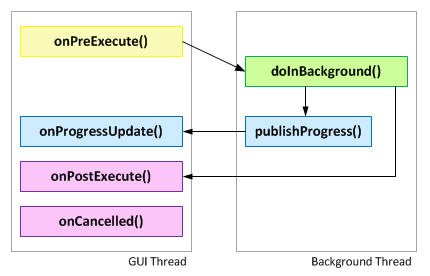
\includegraphics{figs/CicloVidaAsynctask.png}} 
    \caption{Ciclo de vida de Asynctask} 
    \label{fig:CicloVidaAsynctask} 
  \end{center} 
\end{figure}

\subsection{Backup}
\label{subsecc:Backup}

Aunque ya se ha hablado de este tema en el apartado de Google, el tema del backup en Android es un asunto muy importante, la mayoría de aplicaciones tienen algún método para guardar la información que genera el usuario.
Algunas aplicaciones hacen uso del api comentada anteriormente para realizar el backup que ofrece Google, la ventaja de esta propuesta es que la información estará guardada y se podrá recuperar la siguiente vez que el usuario quiera instalar la aplicación.
Otras aplicaciones realizan los backups directamente sobre el dispositivo, usando la tarjeta SD para guardar la información y de esta forma en el caso que el dispositivo se averíe hay una base de datos consistente que se podrá importar.
Al realizar la aplicación, en los primeros casos de uso no se le dio importancia a los backups pero después de circunstancias como fue en mí caso que se me estropeo el móvil, lo hechas en falta. La buena noticia fue que al tener vinculado con Google Calendar todos los exámenes podía saber la fecha que tenían al mirar por la web.
Para que una aplicación sea útil tiene que permitir al usuario llevarse la información entre dispositivos y si por alguna circunstancia se desinstala la aplicación, que pueda instalarla de nuevo con la información que tenía anteriormente.
Hay aplicaciones que usan cuentas de usuario para volver a rellenar la base de datos en local del móvil, pidiéndolas al servidor al momento de instalarlo y así no tener que estar haciendo consultas en cada momento.
Lo que se vio una buena oportunidad era juntar el uso de un api de Google junto con el backup de la aplicación. Por eso se decidió usar Google Drive.

\subsection{Debugging}
\label{subsecc:Debugging}

Cuando se está desarrollando cualquier proyecto la mejor manera de ver si funcionan las cosas es probándolas, en el caso de Android es una de las mejores opciones para que todo funcione como se espera.
Los dispositivos móviles tienen muchas variables que pueden afectar a la aplicación, las versiones o la pantalla son las más generales. Pero no son las únicas, el acceso a internet para una aplicación que tiene que estar sincronizada a los calendarios del usuario es un factor determinante para que vaya bien. La posición en la que se use el dispositivo suele ser un tema complicado de llevar, por eso el apartado de debugging es de los temas más importantes que hay que realizar a la hora de querer publicar una aplicación en el Google Play.
Las aplicaciones que se cuelgan al Google Play no suelen pasar por muchos controles de calidad, así que el desarrollador es el que tiene que ser el control de calidad de su aplicación. Si el propio desarrollador no está satisfecho con su trabajo es que todavía la aplicación no está disponible para salir al mercado.
Si se combina la depuración del programa junto usuarios que puedan probarla y devolver feedback, la aplicación saldrá mucho mejor de lo esperado y mucho antes que si el propio desarrollador tiene que estar haciendo todas las pruebas. 
Hay aspectos que hay que probar cuando se hace el debugging si se está trabajando con un movil. Lo mejor es ir realizando código pequeño y probarlo poco a poco en la aplicación en vez de lanzarse a programar toda la aplicación de golpe y probarlo después, en Android los errores pueden salir por muchos sitios, desde una línea no escrita en el manifest o un botón no declarado a un fallo de asignación en el TextView que se piensa que se está insertando un String y al final era un integer.
 
Por todos estos fallos pequeños de programación si se realiza una aplicación con varios casos de uso el error puede surgir en cualquier función por ese motivo es más sencillo realizarlo de la forma siguiente:
Lo primero realizar la distribución de la vista que tendrá el usuario y probar que se vea adecuadamente.
Una vez se puede ver correctamente en todas las posiciones ya se puede pasar a darle utilidad a los botones por ejemplo. Probar con una notificación estilo Toast que funcionan correctamente los botones y que si se ha programado que salte a otra actividad lo hace sin problemas. También comprobar que pasa al darle hacia atrás y si es lógico que haga eso, ya que las actividades en Android tienen su ciclo de vida e igual no interesa que sigan vivas una vez se ha realizado alguna acción.
Cuando ya las acciones simples funcionan lo siguiente es probar si la función que se ha implementado funciona correctamente para ello en el caso que esa función devuelva  un valor, lo más rápido es añadir al Toast anterior el valor de la función, y añadir un breakpoint en la función a la hora de ejecutar las pruebas conectado al ordenador.
Con ese breakpoint cuando se lance la aplicación en la máquina virtual o el dispositivo físico podrás ejecutar el botón y se parara cuando entre en la función marcada. Se puede ir línea por línea e ir viendo que valores están cogiendo las variables.
Lo mejor en mi opinión para hacer pruebas y no estropear la batería ni el enchufe del móvil es usar una máquina virtual de Android. El problema es el consumo de memoria que tiene el uso de esta opción. Android Studio ofrece su propio administrador de máquinas virtuales de Android. Pero recomiendo usar un software que se llama Genymotion que también está adaptado a Android Studio, la ventaja de este software es que no consume tantos recursos y el móvil va más fluido.
 
En el caso de que se trabaje con servicios de Google las máquinas virtuales no traen por defecto los servicios de Google instalado así que hay que instalarlo en la maquina como si fuera software de terceros. Hay tutoriales por internet e incluso webs que se dedican a subir las apks de Google play para que se puedan instalar dependiendo la versión del móvil.
El funcionamiento es sencillo solo hay que instalar 2 ficheros uno es el ARM Translation installer y el otro son los servicios de Google donde se encuentran Gmail,Google maps, youtube, etc…
Cuando se realizan estos pasos ya se tendrá un móvil Android virtual como el que se tiene físico.
Al trabajar con una máquina virtual las capturas de pantalla y grabaciones son sencillas de hacer. Y el acceso a las carpetas donde se guardan las bases de datos de la aplicación tenemos permisos de super usuarios para entrar y descargar esos datos, cosa que si se prueba en un dispositivo físico se necesitaría rootear el teléfono para hacer lo mismo.
Una vez los casos de uso funcionen como se tenía pensado es hora de subir la aplicación en versión alpha y hacer que los usuarios la prueben.
Para ello algo útil es hacerles un guion a la hora de realizar tareas, ver si lo pueden realizar y si les da algún tipo de fallo.
Aparte del guion es útil que ellos vayan usándola como lo usarían de normal para ver los posibles errores que puedan salir si se lanza al mercado en este momento.
Mediante software que recoge la información de la aplicación como puede ser Google Analytics o Splunk Mint se va revisando los fallos que puede estar dando la aplicación.

 
Durante las pruebas de Baldugenda se usó Splunk Mint, un software que todavía está en desarrollo, pero que funciona muy bien para lo que se necesitaba de la aplicación era captar los errores y decir donde fallaba sin necesitar que el usuario dijera como le había fallado.
Para la instalación dentro del terminal es muy sencilla lo único que hay que hacer es registrarse en splunk mint y una vez registrado crear un proyecto, agregar la librería mediante gradle o metiéndola en el proyecto.
Y después seguir los pasos que marcan en la web para hacer las llamadas a sus servicios.
Ofrece un seguimiento muy bueno dentro de la aplicación, se puede programar para que cuando un usuario pulse un botón esa acción quede recogida en su página web y después lo mostrara cuando entremos, también realiza notificaciones al email que le digamos. 
El manejo es muy sencillo se separa en 3 pestañas, la primera es donde está la información de las conexiones y de los dispositivos que tienen instalada la aplicación, la segunda pestaña es para los errores que se dan y te permite filtrarlos por fecha y te muestra un gráfico de tiempo la cantidad de errores que se han producido y la versión que en la que se ha producido el error. Y la tercera pestaña es para las configuraciones del proyecto, Splunk mint permite vincular con el proyecto que se suba a github y hacer comentarios dentro del código, en el caso que se resuelva algún error se le puede decir a splunk mint que escriba en github que se ha resuelto y en que versión ya no se produce.

\begin{figure}[H] 
  \begin{center} 
    \scalebox{0.8}{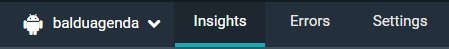
\includegraphics{figs/SplunkMintMenu.png}} 
    \caption{Splunk Mint Menú} 
    \label{fig:SplunkMintMenu} 
  \end{center} 
\end{figure}

Los errores aparecen de la siguiente manera y es posible entrar a ellos y ver línea a línea por donde ha pasado el programa hasta llegar al error.

\begin{figure}[H] 
  \begin{center} 
    \scalebox{0.8}{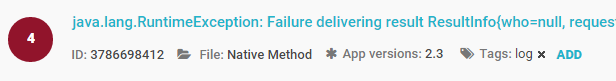
\includegraphics{figs/ErrorSplunkMint.png}} 
    \caption{Error en Splunk Mint} 
    \label{fig:ErrorSplunkMint} 
  \end{center} 
\end{figure}

También se puede configurar para que envié los errores al email que queramos.

\begin{figure}[H] 
  \begin{center} 
    \scalebox{0.8}{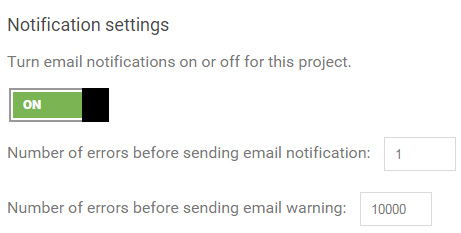
\includegraphics{figs/ConfiguracionSplunkMint.png}} 
    \caption{Configuración  Splunk Mint} 
    \label{fig:ConfiguracionSplunkMint} 
  \end{center} 
\end{figure}

Y se trabaja muy bien en el caso que sea un grupo de personas da la posibilidad de permitir ver los errores a un equipo de proyecto y enviar las notificaciones.

\subsection{Control de versiones}
\label{subsecc:Control de versiones}

Al desarrollar en Android una parte importante es mantener siempre accesible el código y saber qué cambios se han realizado, un programa, da igual el lenguaje que se esté usando y el dispositivo al que vaya enfocado es igual que un libro, no se redacta o en el caso de aplicaciones se implementa de un día para otro. Por este motivo es útil siempre usar el control de versiones para tener constancia de los cambios efectuados y si en algún momento se necesita volver a una versión anterior es más fácil realizarlo que empezar a escribir todo de nuevo, pudiendo ocasionar perdida de código por el camino y el fallo del programa.
En el caso de Android, su IDE, Android Studio facilita enormemente el trabajo con el control de versiones ya que trae incorporado opciones que permiten subir directamente el código a github. El único requisito que pide es tener una cuenta de github y ya estaría funcionando la subida de código con su respectivo control de versiones.
Los puntos positivos de usar el control de versiones de github es que aparte de saber el propio desarrollador lo que ha ido generando día tras día, es un buen método para que las demás personas conozcan tus trabajos y vean si eres una persona periódica en las tareas de programación.
El propio Google usa github para tener sus proyectos de ejemplo de los apis que distribuye. Así que habituarse a usar esta herramienta es un buen comienzo para ver cómo trabajan los demás desarrolladores.
Aparte github tiene plugin para multiples programas como puede ser los de procesador de latex, una manera útil de realizar la memoria y subirla al repositorio y tenerla segura.
En el caso de usar Word 2013, ofrece también la posibilidad de marcar el control de cambios realizados, no es tan útil como github que aparte de guardarte los cambios puedes viajar por las versiones del fichero subido pero, por lo menos se tendrá constancia de los cambios realizados ese día.
 
Igual que Github hay otros repositorios interesantes como puede ser gitlab, gitorious o bitbucket
Cada uno tiene sus ventajas con respecto a los otros, github por ejemplo tiene solo repositorios públicos si se quiere usar de forma gratuita, en el caso que se quiera repositos privados hay que pagar.
En bitbucket y los rivales de github aprovechan eso de los repositorios privados y ofrecen uno o dos repositorios privados de forma gratuita al crear la cuenta.
De esta forma los desarrolladores pueden estar desarrollando código sin la sensación que la competencia se lo pueda quitar.
Cuando se está implementando código una buena forma de hacerlo es ir subiendo el código que funcione únicamente, por mucho que se estén haciendo pruebas, el repositorio no tiene que ser un lugar donde se guarda el código que igual un día se use. 
La forma de ver el repositorio tiene que ser un lugar donde guardar el código que ya se ha probado y funciona y poco a poco ir aumentándolo hasta tener un programa consistente que aunque de fallos en ciertos momentos por lo menos son fallos de las últimas modificaciones realizadas.
También se puede ver como una manera de acceder al código sin tener que llevarlo siempre en el USB, puedes estar trabajando en el ordenador de la facultad y cuando se acaba subirlo al repositorio, al llegar a casa descargarlo y seguir trabajando. 
En la situación de Baldugenda no era preciso usar github como método de trabajo en equipo ya que el equipo estaba formado por una sola persona, pero aun y todo era una buena forma de llevar al día el tiempo que había llevado hacer cada implementación y que se había ido haciendo en cada ciclo del proyecto.
Si una aplicación la van a realizar más personas es casi imprescindible el uso de herramientas como github, ya que no se puede estar exportando el proyecto y compartiéndolo por correo con cada modificación que se haga, porque sería una confusión enorme.
Un problema de usar github es que todos los miembros del equipo tienen que saber usarlo, sino puede llevar a problemas de código corrupto al subirse o fallos así que no permitirían subir el código. Pero una vez aprendido a usar github el uso que se le puede dar es enorme, ahora permite crear páginas web explicando el proyecto que esta subido y permitiendo que otros se lo descarguen o que hagan copias del proyecto en sus repositorios.
El funcionamiento de github es por la consola si no se va a usar el plugin de Eclipse o Android Studio, aunque, se ha desarrollado aplicaciones propias para Mac  y para Windows, que hacen más fácil e interactivo la subida y descarga de los proyectos.

\subsection{Problemas al desarrollar en Android}
\label{subsecc:Problemas al desarrollar en Android}

Ya se ha hablado de los puntos importantes al crear un proyecto en Android y cosas que hay que tener en cuenta. 
Al desarrollar en Android hay ciertos momentos que fallan cosas y no se encuentra solución, en este apartado se hablara de los casos que han sucedido en Baldugenda y como se han solucionado.
Uno de los casos más comunes es cuando se importa un proyecto de github o eclipse. La mayoría de veces el IDE no detecta bien las librerías asociadas al proyecto y marca errores tanto de vistas como de la clase R de Android. 
Algunas maneras de solucionarlo es instalando las apis que requiere el proyecto, al no tenerlas descargadas e instaladas en el ordenador donde se está implementando esto ha podido hacer que falle la compilación y ha hecho que se vuelva loco Android Studio.
Otra solución desesperada es dentro del menú build de Android Studio la opción clean, con esto se limpiara la compilación anterior y realizara una nueva.
Un problema muy común para los que desarrollan en Eclipse son las modificaciones en el manifest o xml de vistas, hay muchas veces que se genera una actividad nueva y se olvida que para usarla tiene que estar en el manifest apuntada.
Con Android Studio este problema no pasa en gran medida ya que da la opción de generar todo de golpe, genera los layouts, modifica el manifest y genera los menus si se quiere solo dándole a un botón.
Si se es nuevo con Android como era yo al empezar la aplicación, no se conoce tan a fondo los entresijos  que depara Android a la hora de programar, uno de ellos es el uso de los servicios web.
Acostumbrado a realizar las llamadas de los servicios web donde quisiera, un error fue meterlo directamente en la actividad, al ejecutar la aplicación se bloqueaba y el debugging llevaba a unas clases creadas por Android.
Buscando por internet explicaban que en Android toda acción que haga que la pantalla se bloqueara durante un tiempo no estaba permitida hacerla en el hilo principal de la actividad.
Ese descubrimiento fue muy útil, ya que con eso aprendí  muchas cosas sobre los hilos en Android y las tareas asíncronas.
 
Antes se ha hablado del uso de máquinas virtuales, uno de los problemas que tiene usar máquinas virtuales son los recursos del ordenador físico que las está moviendo. En más de una ocasión se ha quedado el ordenador sin memoria por tener el Android Studio y la máquina virtual abierta, el único consejo que hay al respecto es intentar no usar máquinas virtuales muy pesadas, cuanto más alta es la api y mayores recursos se le asignan a la maquina más pesada es y más va a exigir.
Android Studio es un IDE potente para desarrollar aplicación Android el problema de esto es que al ser potente también exige mucho. Si se quiere desarrollar en Android se necesita un equipo que tenga suficiente memoria para no quedarse esperando porque se ha quedado parado al compilar el Gradle.

